\section{Wireless Platform}
\label{sec:wireless}
  \subsection{Key Factors and Components}

\begin{frame}{Hardware Description}
\setbeamercovered{dynamic}%Makes the text appear before it presents nice!!!! 
    \begin{columns}[t] % contents are top vertically aligned
      \begin{column}[T]{5cm} % each column can also be its own environment
        \begin{itemize}
            \item<+-| alert@+> Single component of the base winding Figure:~\autoref{fig:structure}.
            \item<+-| alert@+> Receiver platform values Figure:~1b.
            \item<+-| alert@+> Worst coupling position Figure:~1c.
            \item<+-| alert@+> Best coupling position Figure:~1d.
          \end{itemize}  
      \end{column}
    \begin{column}[T]{5cm} % alternative top-align that's better for graphics
      \begin{figure}
        \only<1>{%
        \vspace*{-1.5cm}
          \begin{subfigure}[b]{1.0\linewidth}
            \caption{Single Transmitter Winding} \label{fig:structure}
            \hspace*{-1cm}
            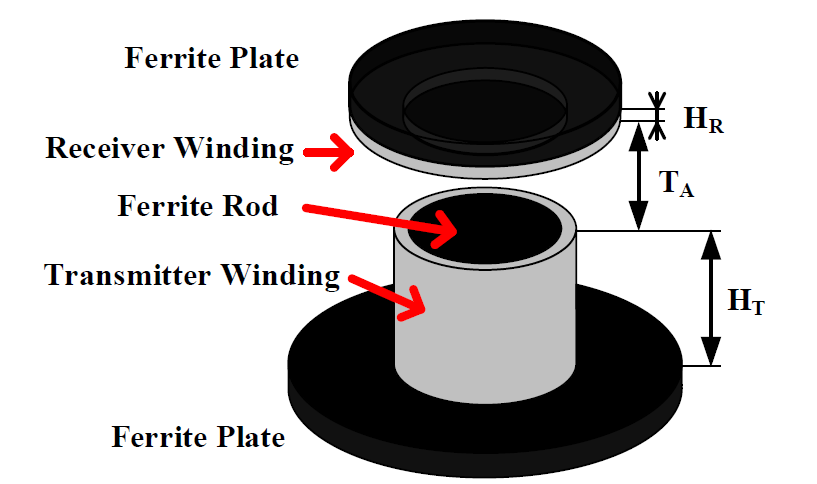
\includegraphics[width=7.0cm,height=5cm]{./png/structure}
            %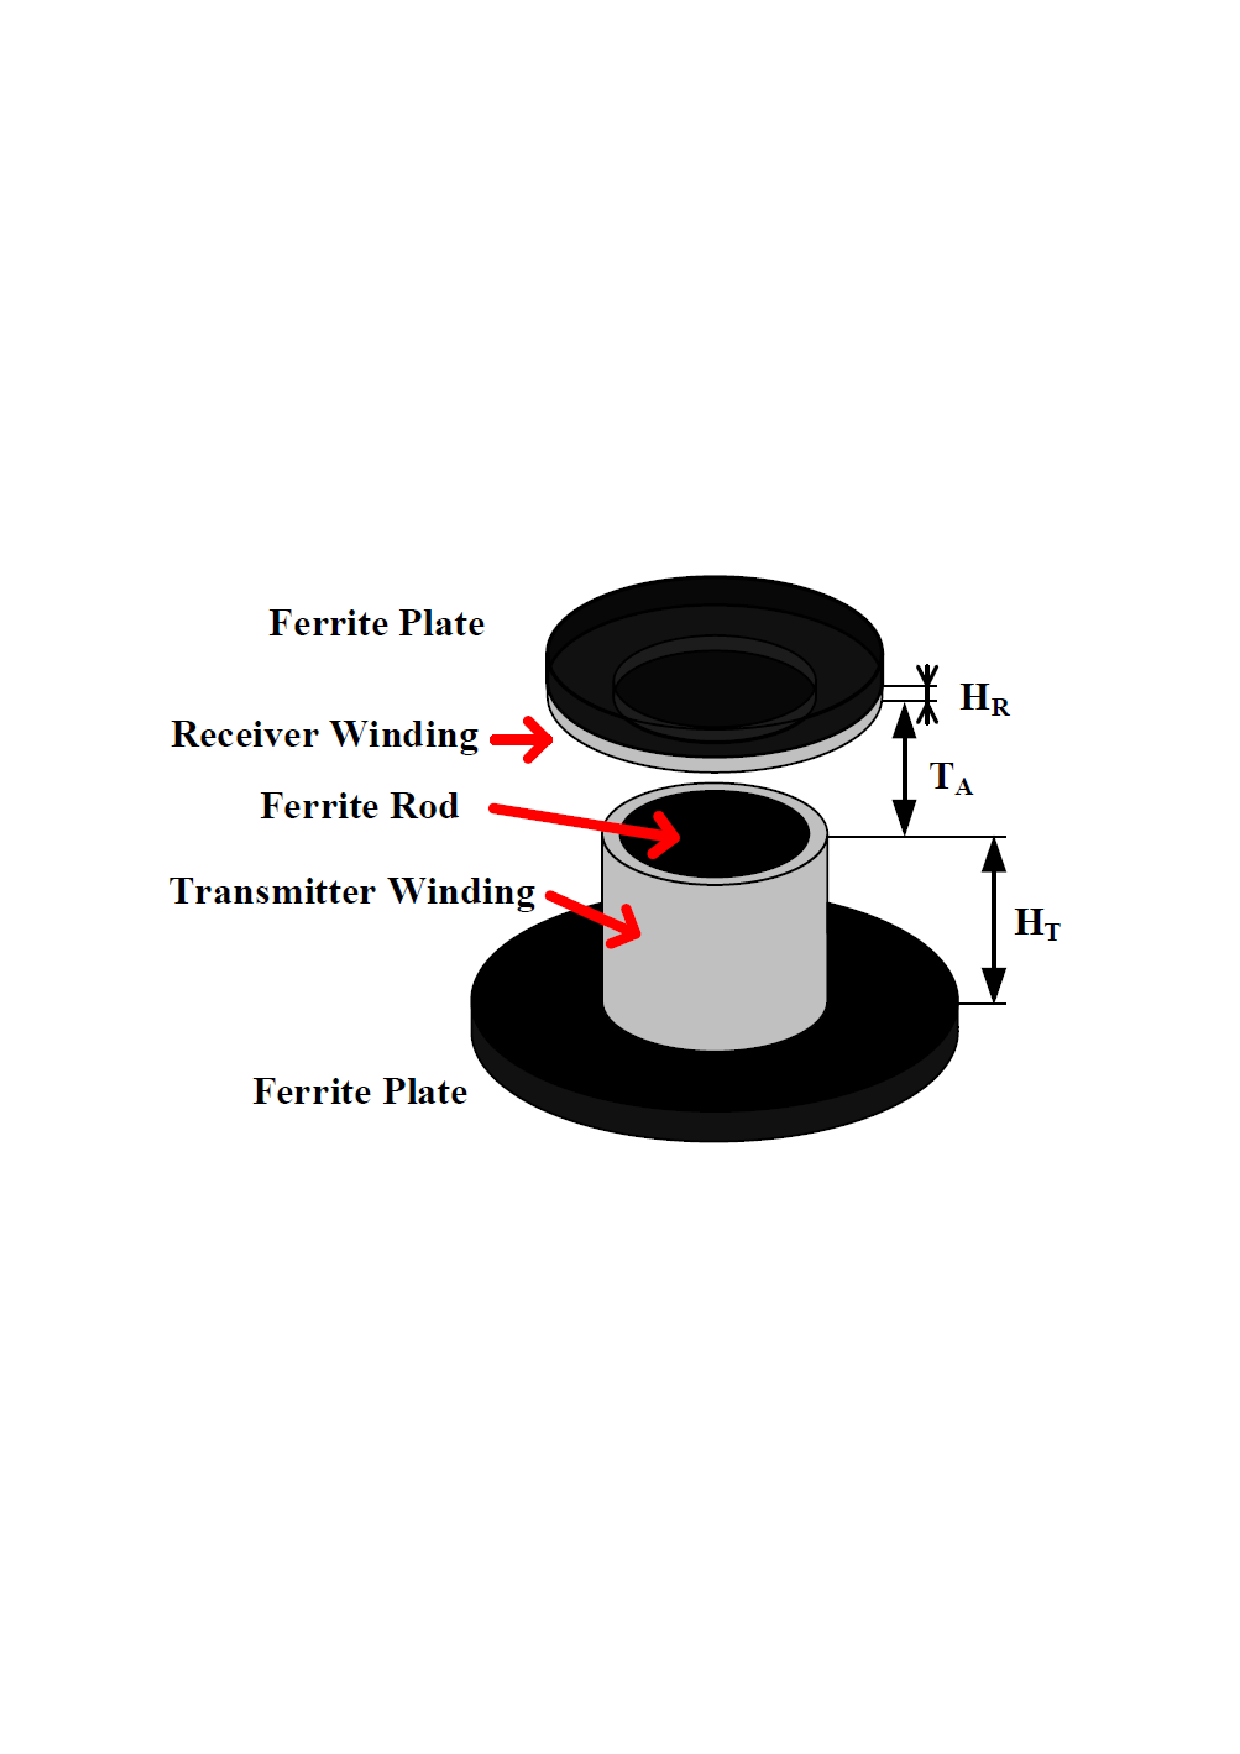
\includegraphics[width=\textwidth]{./pdf/core}
            %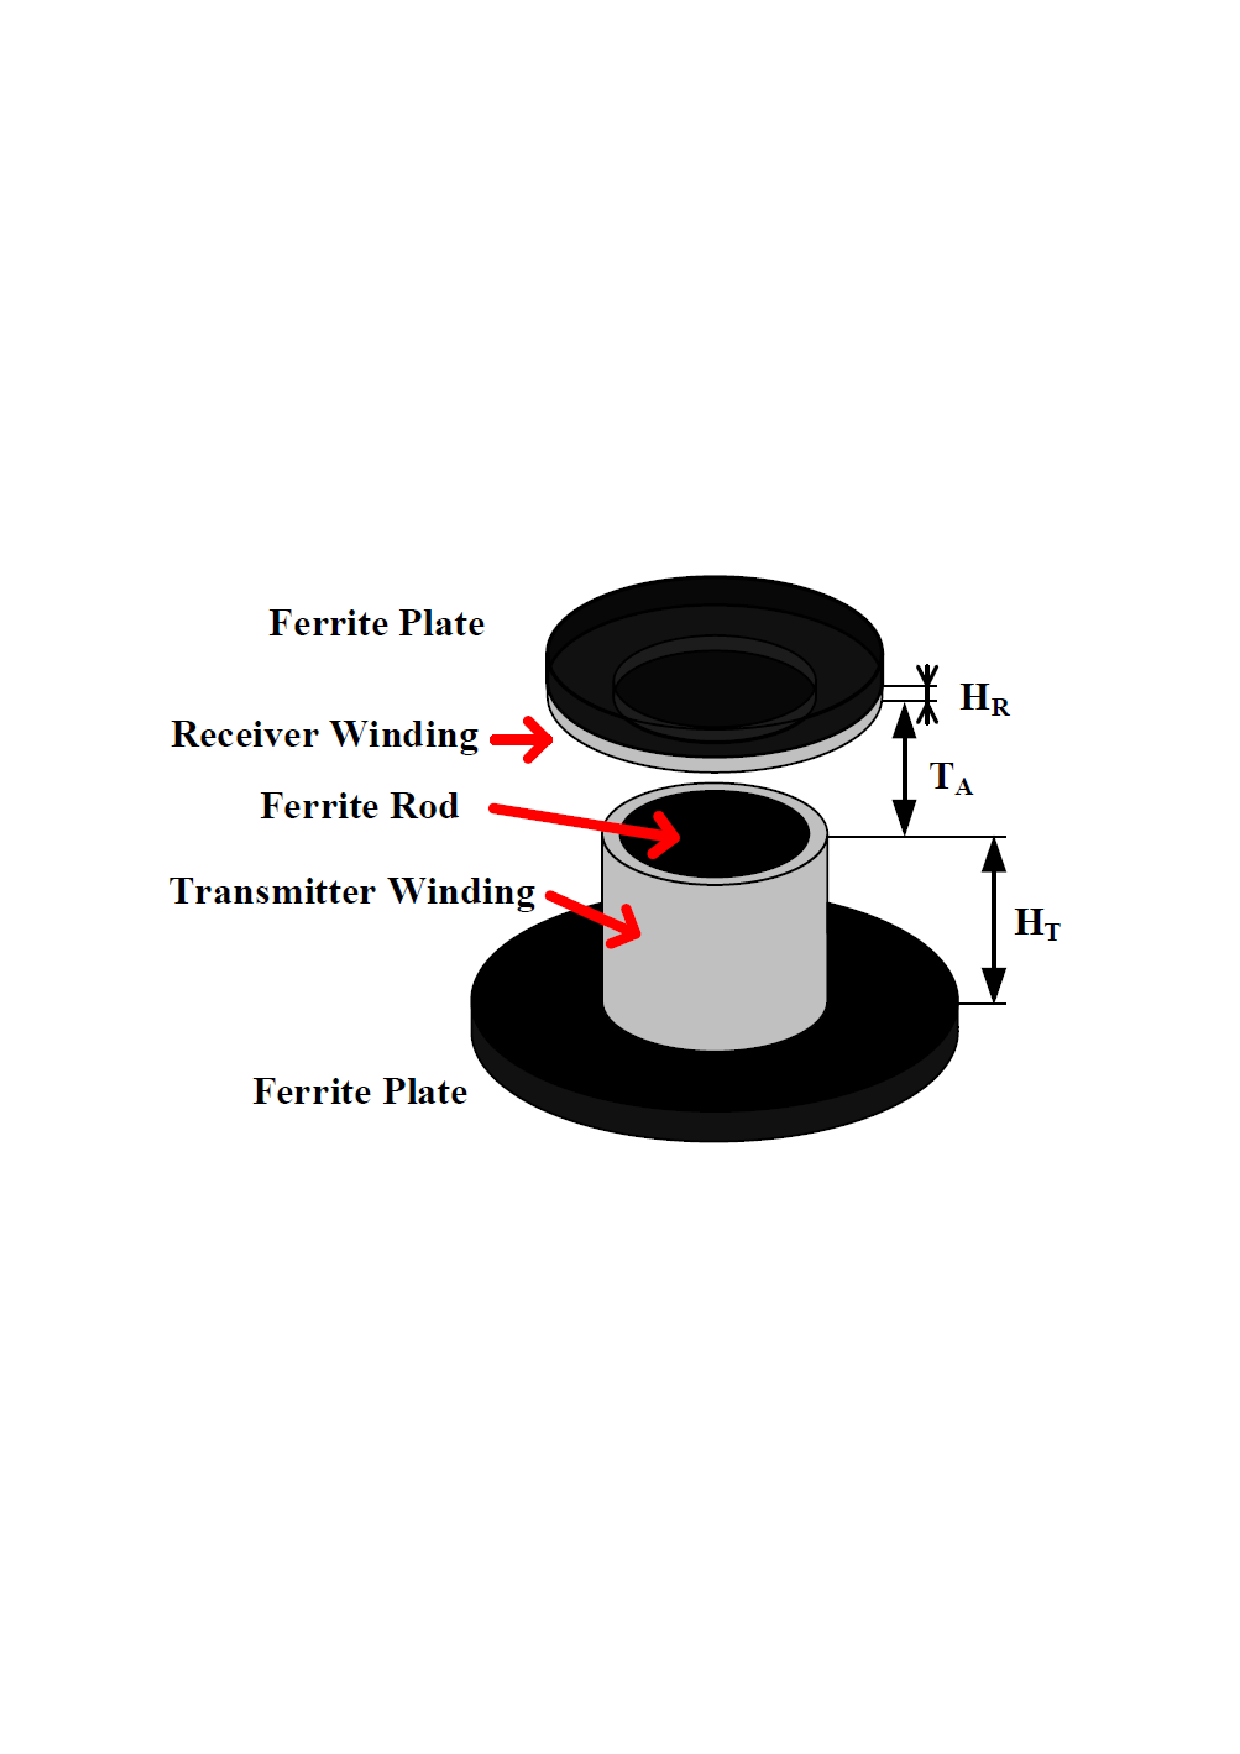
\includegraphics[height=9.5cm]{./pdf/core}
            \vspace*{-0.6cm}
          \end{subfigure}\hfill
        }
        \only<2>{%
          \vspace*{-1.5cm}
          \begin{subfigure}[b]{1.0\linewidth}
            \caption{Receiver Parameters Values} \label{fig:receiver}
            \hspace*{-0.5cm}
            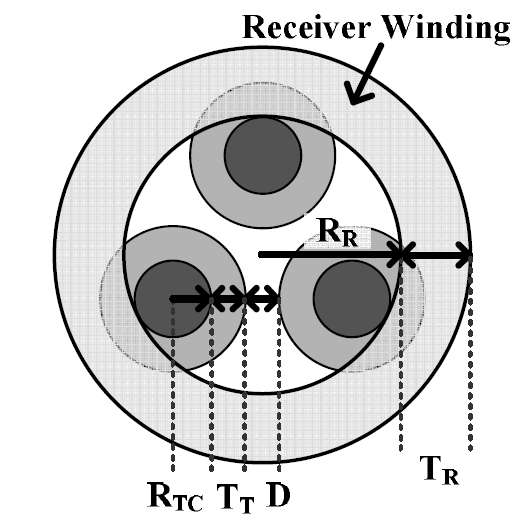
\includegraphics[width=5.5cm,height=5cm]{./png/receiver}
          \end{subfigure}
        }
        \only<3>{%
          \vspace*{-1.5cm}
          \begin{subfigure}[b]{1.0\linewidth}
            \caption{Worst Coupling Positioning} \protect\label{fig:worst}
            %\hspace*{1cm}
            \vspace*{0.1cm}
            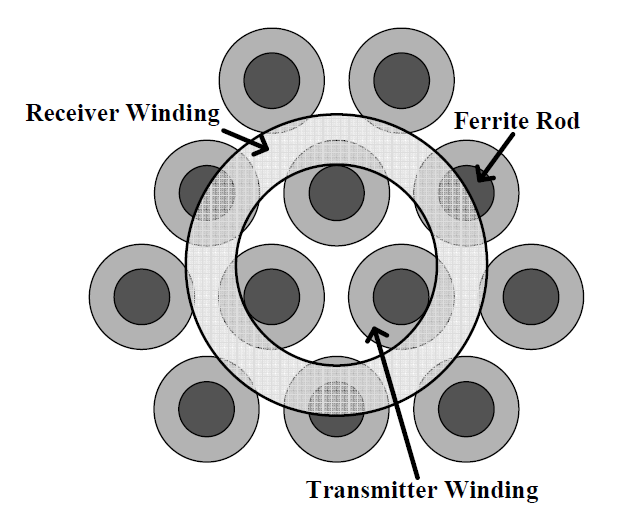
\includegraphics[width=5.5cm,height=5cm]{./png/worst}
          \end{subfigure}
        }
        \only<4>{%
          \vspace*{-1.5cm}
          \begin{subfigure}[b]{1.0\linewidth}
            \caption{Best Coupling Positioning} \protect\label{best}
            %\hspace*{0.5cm}
            \vspace*{0.1cm}
            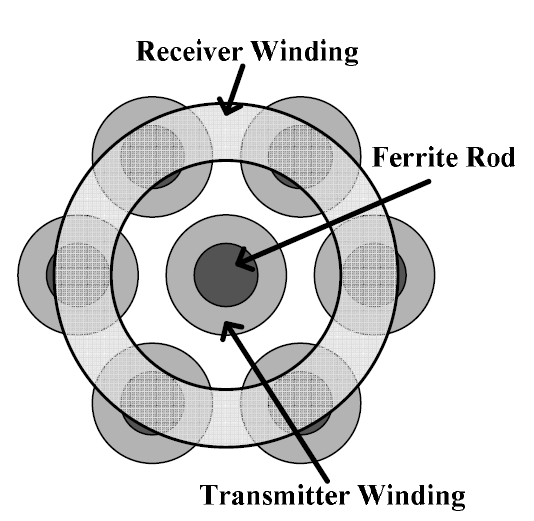
\includegraphics[width=5.5cm,height=5cm]{./png/best}
          \end{subfigure}
        }
      \captionsetup{justification=centering} %Center a two line caption
      \caption{Project Positioning Analysis} \protect\label{fig:5}~\cite{wsn}
    \end{figure}
    \end{column}
  \end{columns}
\end{frame}

\subsection{Best and Worst Performance Based on Positioning}

\begin{frame}{Theory Vs Practical Experimentation}
\setbeamercovered{dynamic}%Makes the text appear before it presents nice!!!! 
    \begin{columns}[t] % contents are top vertically aligned
      \begin{column}[T]{5cm} % each column can also be its own environment
        \begin{itemize}
            \item<+-| alert@+> Best Position Simulation (\ding{108})
            \item<+-| alert@+> Worst Position Simulation (\alert{\ding{110}})
            \item<+-| alert@+> Best Position Measured (\ding{108})
            \item<+-| alert@+> Worst Position Measured (\alert{\ding{110}})
            \item<+-| alert@+> Simulation is a perfect line, in ``\alert{Theory}''
            \item<+-| alert@+> Practical measuring shows ``\alert{150KHz}''!
        \end{itemize}
      \end{column}
    \begin{column}[T]{5cm} % alternative top-align that's better for graphics
      \begin{figure}
        \vspace*{-10pt}
        \centerline{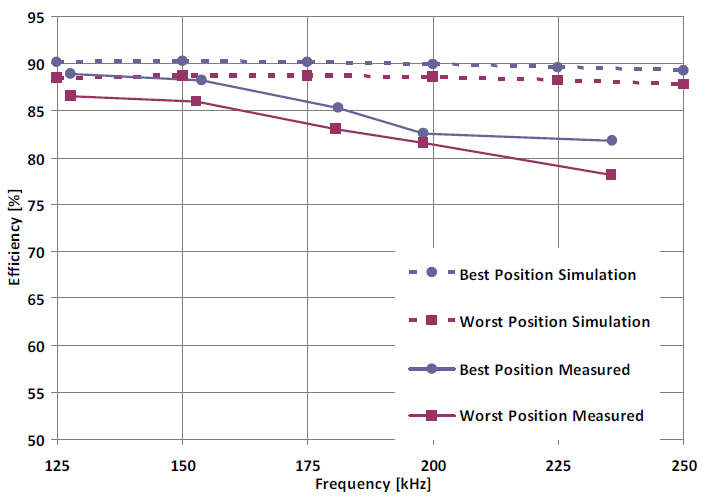
\includegraphics[scale=0.7]{./png/efficiency}}
        \vspace*{10pt}
        \captionsetup{justification=centering} %Center a two line caption
        \caption{Simulation Vs Real Time Efficiency~\cite{wsn}}
        %\includegraphics[options]{path_to_image}syntax
      \end{figure}
    \end{column}
  \end{columns}
\end{frame}
